%% ****** Start of file template.aps ******%
%%
%%
%%   This file is part of the APS files in the REVTeX 4 distribution.
%%   Version 4.0 of REVTeX, August 2001
%%
%%
%%   Copyright (c) 2001 The American Physical Society.
%%
%%   See the REVTeX 4 README file for restrictions and more information.
%%
%
% This is a template for producing manuscripts for use with REVTEX 4.0
% Copy this file to another name and then work on that file.
% That way, you always have this original template file to use.
%
% Group addresses by affiliation; use superscriptaddress for long
% author lists, or if there are many overlapping affiliations.
% For Phys. Rev. appearance, change preprint to twocolumn.
% Choose pra, prb, prc, prd, pre, prl, prstab, or rmp for journal
%  Add 'draft' option to mark overfull boxes with black boxes
%  Add 'showpacs' option to make PACS codes appear
%  Add 'showkeys' option to make keywords appear
\documentclass[aps,prl,preprint,groupedaddress]{revtex4}
%\documentclass[aps,prl,preprint,superscriptaddress]{revtex4}
%\documentclass[aps,prl,twocolumn,groupedaddress]{revtex4}

% You should use BibTeX and apsrev.bst for references
% Choosing a journal automatically selects the correct APS
% BibTeX style file (bst file), so only uncomment the line
% below if necessary.
%\bibliographystyle{apsrev}
\usepackage{graphicx,csquotes}

\begin{document}

% Use the \preprint command to place your local institutional report
% number in the upper righthand corner of the title page in preprint mode.
% Multiple \preprint commands are allowed.
% Use the 'preprintnumbers' class option to override journal defaults
% to display numbers if necessary
%\preprint{}

%Title of paper
\title{Planetary Transparency Protocol (PTP): \\
Decentralizing the Earth Analytics Market}

% repeat the \author .. \affiliation  etc. as needed
% \email, \thanks, \homepage, \altaffiliation all apply to the current
% author. Explanatory text should go in the []'s, actual e-mail
% address or url should go in the {}'s for \email and \homepage.
% Please use the appropriate macro foreach each type of information

% \affiliation command applies to all authors since the last
% \affiliation command. The \affiliation command should follow the
% other information
% \affiliation can be followed by \email, \homepage, \thanks as well.
\author{Pavel Machalek}
%\email[pavel@spaceknow.com]{}
%\homepage[]{Your web page}
%\thanks{}
%\altaffiliation{}
\affiliation{}

%Collaboration name if desired (requires use of superscriptaddress
%option in \documentclass). \noaffiliation is required (may also be
%used with the \author command).
%\collaboration can be followed by \email, \homepage, \thanks as well.
%\collaboration{}
%\noaffiliation

\date{\today}

\begin{abstract}
We present a decentralized protocol for analyzing and trading geospatial intelligence on each of the 510 million square kilometers of the Earth's surface.  Earth Observation (EO) industry has been plagued for decades by a market mismatch between supply of imagery (scarce, expensive, regulated) and demand for geo-spatial information from individuals, corporates and sovereign governments (fragmented demand, customized specifications, unexplored applications of EO data). Even in the advanced Internet age with full GPS and GSM penetration, it is difficult and expensive to know what is happening on any one kilometer square grid on Earth in real time.\\
The open-sourced Planetary Transparency Protocol (PTP) aims to address this market inefficiency by standardizing 1) access to all the commodified providers of EO imagery and 2) creating a de-centralized market place for exchange of analytics, information and metadata for each square kilometer of the Earth's surface grid ( 1 sq.km worth of datafeed per year = 1 PTP unit of value).\\
Consumers of information (demand) will ask for data, analytics and informations for each grid and providers of data, analytics and information will match the demand for each individual grid with supply of information in a completely decentralized manner.  \\
The marketplace will be seeded by the issuance of 510 million PTP coins, one for each grid. Each grid accumulates an encrypted, uncensorable, distributed and tradable datastream of geospatial information. 
\end{abstract}

% insert suggested PACS numbers in braces on next line \pacs{}
% insert suggested keywords - APS authors don't need to do this
%\keywords{}

%\maketitle must follow title, authors, abstract, \pacs, and \keywords
\maketitle

% body of paper here - Use proper section commands
% References should be done using the \cite, \ref, and \label commands
\section{Introduction}
Earth sensing has been used for decades by governments and large multinationals to remotely scan the Earth and derive useful information about the industrial and military activity of nation states, corporations and industries \cite{campbell2011introduction}. Analysis of satellite imagery has a wide variety of uses: from tracking growth of cities, to environmental management to tracking illegal logging and human rights abuses monitoring. The ability to obtain and process satellite imagery and distribute the obtained information has been limited so far to sovereign actors, corporates and large educations institutions. \\

% Put \label in argument of \section for cross-referencing
%\section{\label{}}
\begin{figure}[h]
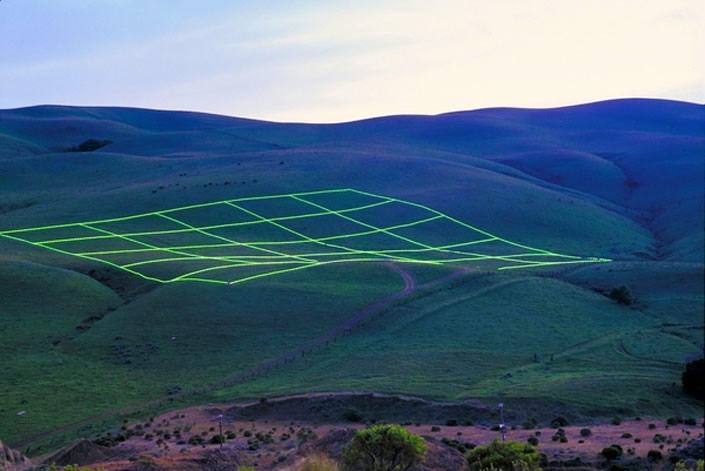
\includegraphics[width=0.5\linewidth]{earth_grid_01.jpg}
\caption{One kilometer square grids. Art by Stuart Williams.}
\end{figure}
Planetary Transparency protocol matches consumers of geospatial information such as information from analyzed satellite imagery with producers and analyzers of such data. By introducing liquidity and locations specific pricing for monitoring each 1km $\times$ 1km Earth grid, market and pricing discovery mechanism will allow users and consumers to signal where and what they would like imaged. We introduce a medium of exchange \cite{friedman1991island} of PTP coin, which denotes a subscription to monitor and analyze 1 square kilometer of Earth's surface for a whole year. Each PTP coin will enable the bearer to monitor and analyze one square kilometer for a given year from the providers who choose to provide the data for that given grid at a given process set by the market for that specific grid. 

\section{The grid}
\begin{figure}[!h]
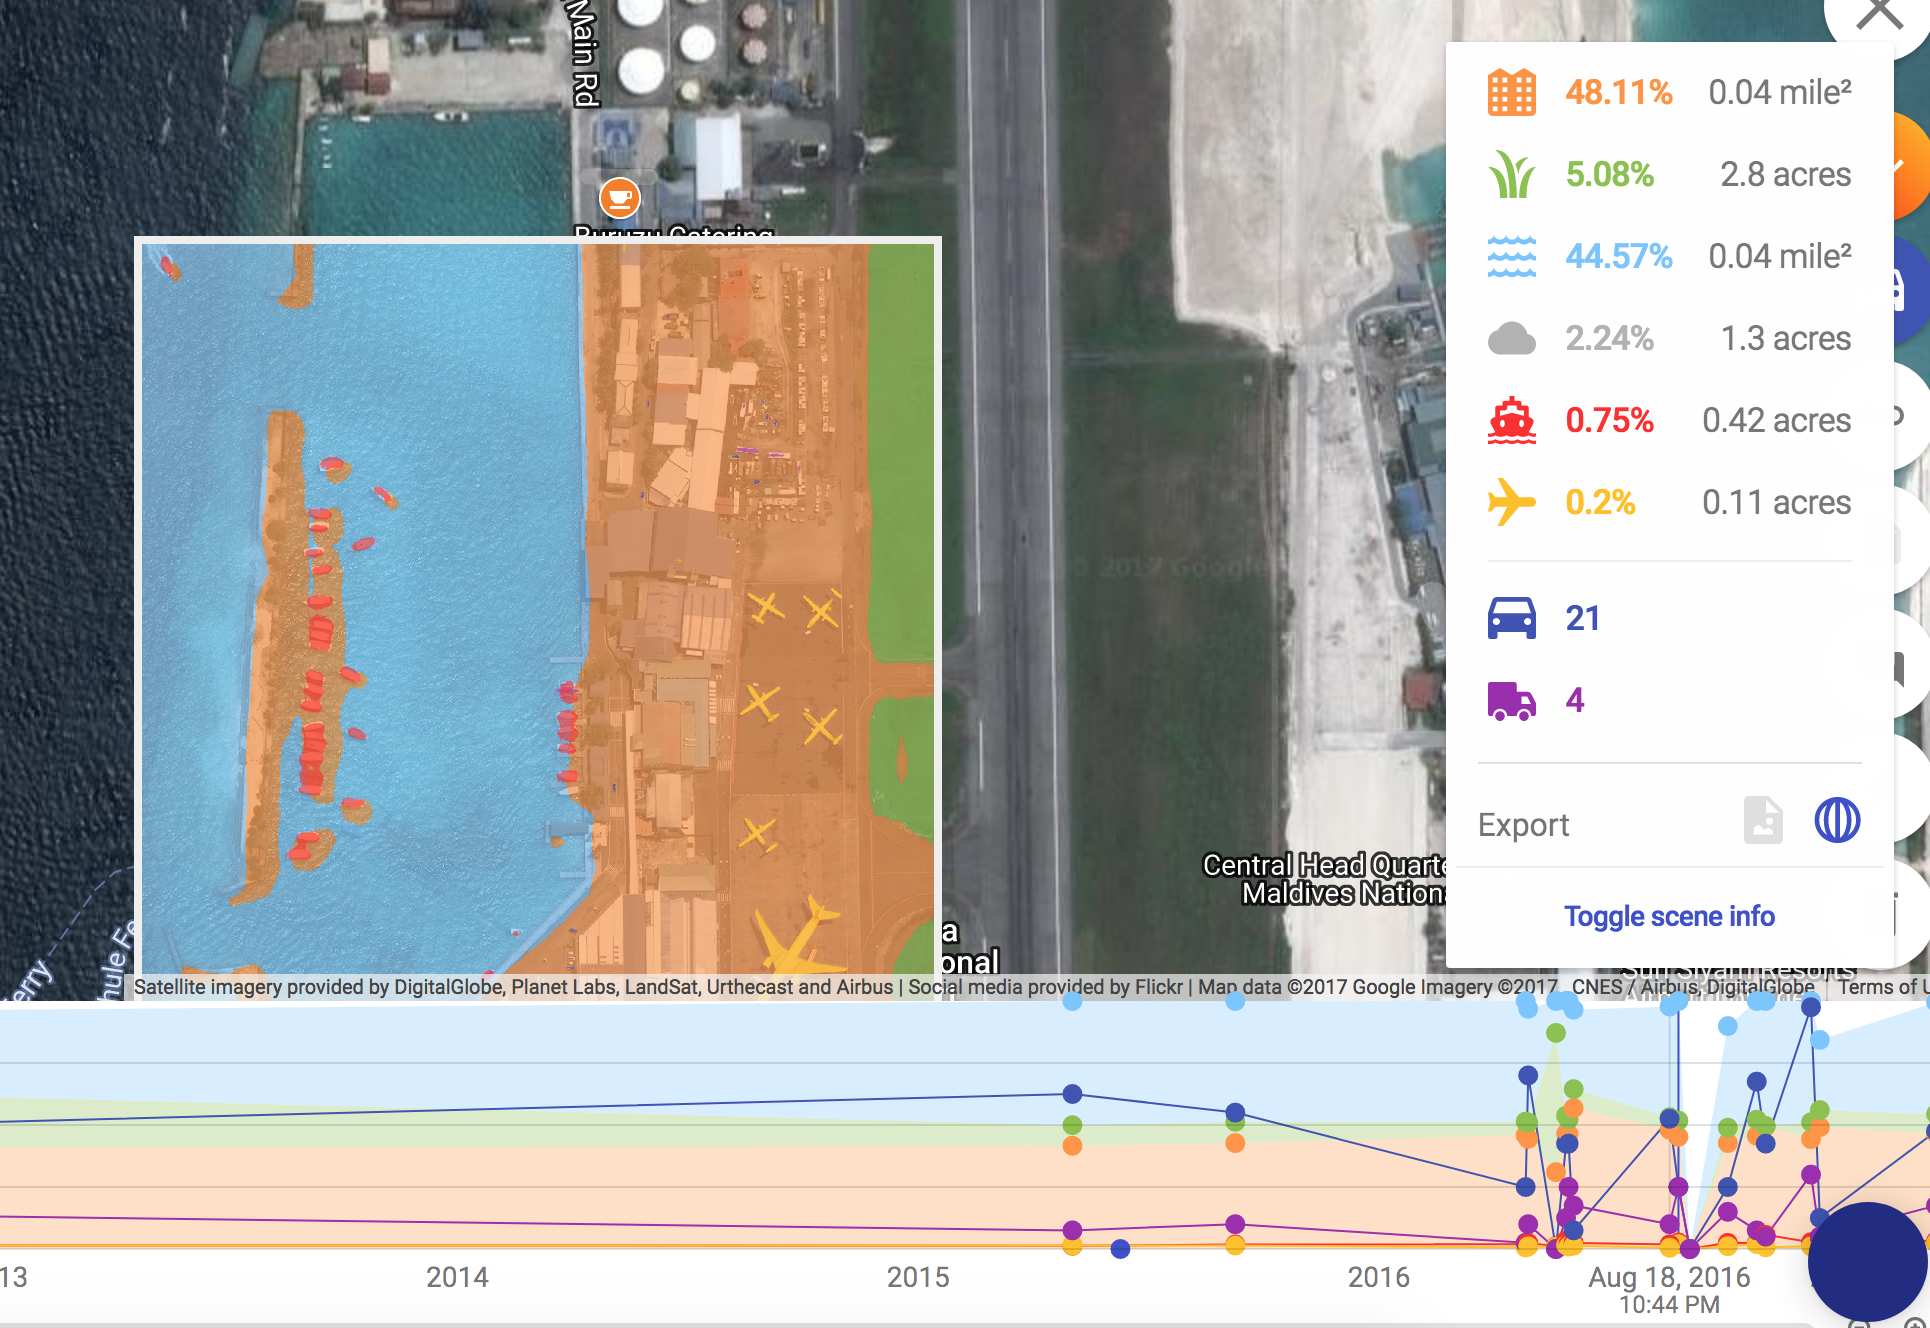
\includegraphics[width=0.8\linewidth]{computing_grid.png}%
\caption{\label{sk_grid} \small{Examples of centralized analytical system by Spaceknow. Note the satellite image in the white rectangle "the grid" overlaid by orange, blue and green colors which denote man-made, water and natural landuses as analyzed by the Convolutional Neural Network. Furthermore note the aircraft, ship, cars and trucks detections denoted by their respective colors in the legend. }}
\end{figure}

The basic computing unit of PTP is one kilometer by one kilometer computing grid on the Earth's surface (for a centralized, commercially controlled example see Fig. \ref{sk_grid}). Each grid represents a localized market for exchange of data storage of geo-spatial information (satellite imagery, vector data, social media,...) and processing of such geospatial information by independent Processors, who will submit the results back to the decentralized storage associated with each grid \cite{benet2014ipfs}.
Buyers will ask to subscribe to geospatial data feeds (object counts, vectorized outputs of deep learning algorithms, social media feeds, localized news feeds) with PTP coins and the providers of analysis and data will have an incentive to be paid a subscription fee in each grid. The subscription fee paid per each grid will vary and will be set by supply and demand. 




\section{Proof-of-Subscription}
\begin{figure}[!h]
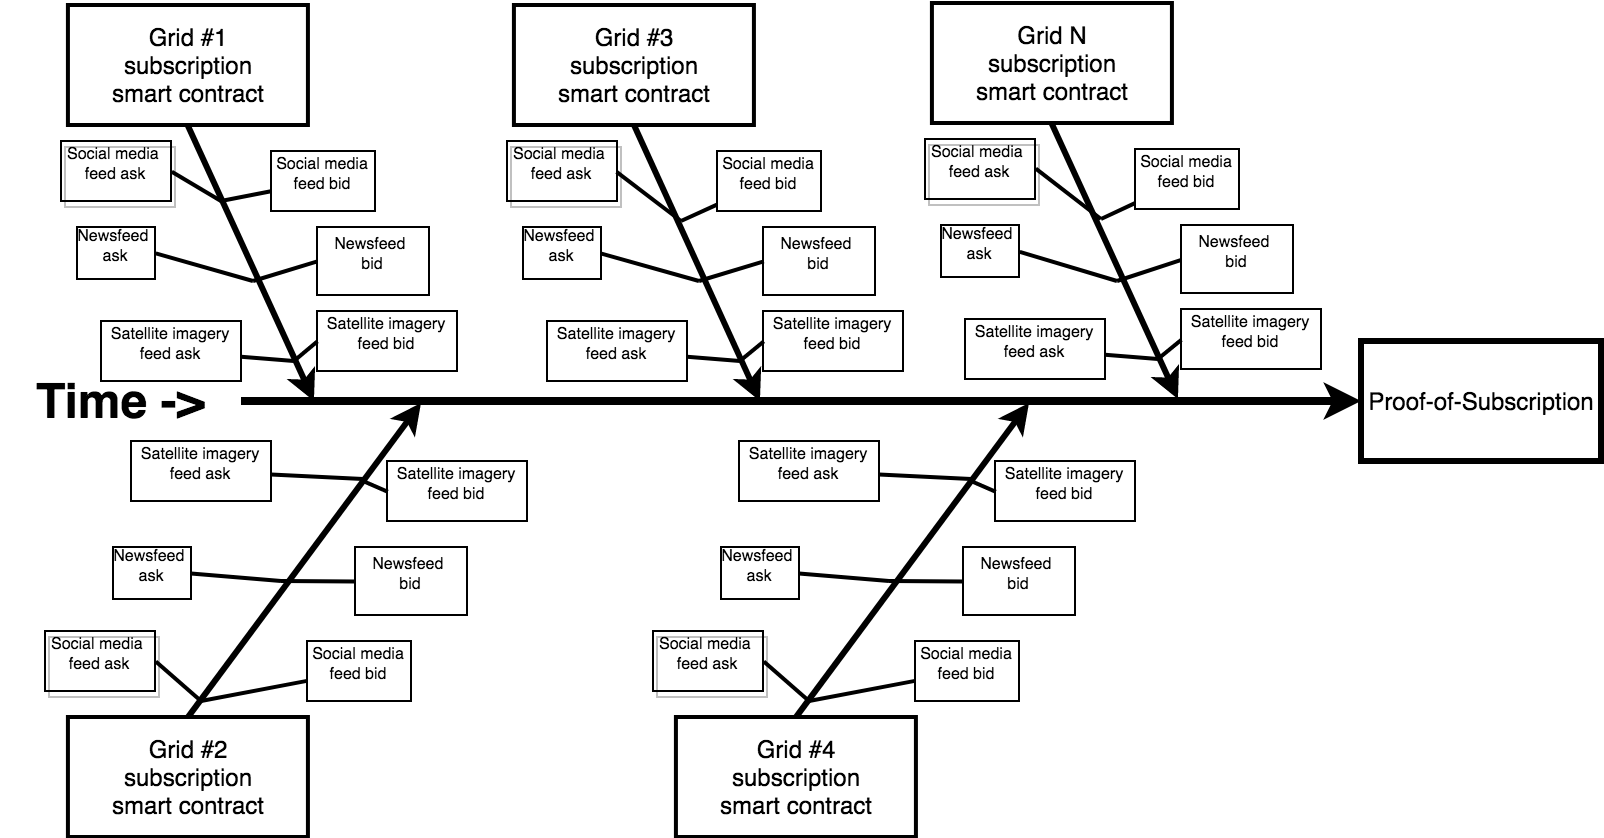
\includegraphics[width=0.8\linewidth]{Proof-of-Subsription__1_.png}%
\caption{Proof-Of-Subscription concept}
\end{figure}

\blockquote{\it{[Hiro has] been putting a lot more emphasis on his auxiliary emergency backup job: freelance stringer for the CIC, the Central Intelligence Corporation of Langley, Virginia. Millions of other CIC stringers are uploading millions of other fragments at the same time. CIC's clients, mostly large corporations and Sovereigns, rifle through the Library looking for useful information, and if they find a use for something that Him put into it, Hiro gets paid.}\cite{stephenson2014snow}}




The central concern in the Planetary transparency protocol is who and when is a holder of PTP coins subscribed to a particular datafeed on a particular grid. In other words who gets which information from which provider and when and where. The subscription ask/bid and matching process will be handled by Ethereum based smart contract which will match providers with consumers of data on a grid and handle initialization, continuance and terminations of datafeeds.  





\section{Incentive}
After the first 510 million PTP coins are distributed during the ICO, the holders of PTP coins can subscribe to datafeeds for each grid. Initially there might be few, if any, providers of information datafeeds in each grid. Holders of PTP coins can place "asks" in each grid that demonstrate their interest in subscribing to a particular social media, satellite imagery or another processed datafeed for that grid. When a subscription from a user is activated the chosen amount of PTP coins are deposited into the grid escrow and are publicly visible. The more interest there is in a particular grid the more funds will be held in that grid's escrow and entice providers of information subscriptions to "bid" for the "asks" and start receiving the subscription funds from that grids escrow. Any subscriber can stop his subscription at any time and withdraw his funds from that grid's escrow, just as much as any provider can stop providing services to each grid. 

\begin{figure}[h]
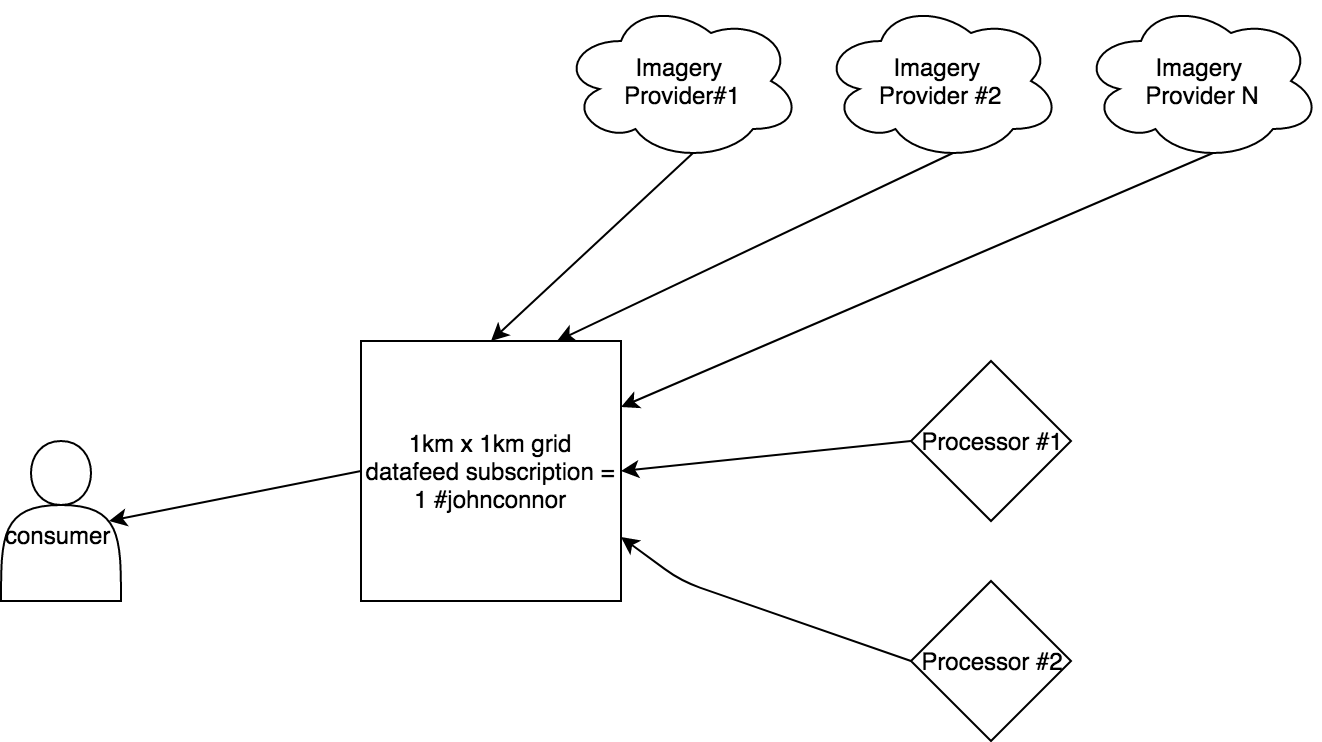
\includegraphics[width=0.5\linewidth]{CIC.png}%
\caption{Structure of the marketplace}
\end{figure}

\section{Censorship resistance}
Currently the world's remote sensing platforms (satellite imaging) are tightly controlled and regulated by the Cold War's sovereign super powers such as USA, Russia and different entities in the EU using tools such as "shutter-control", "exclusion zones" and resolution and time delays on the provenance and distribution of satellite imagery and advanced imagery analytics products\footnote{http://spacenews.com/pentagon-list-could-clear-the-way-for-licensing-of-advanced-commercial-imaging-systems/}.  Planetary Transparency Protocol (PTP) explicitly aims to wrest control of the space imaging and analytics away from sovereign governments and decentralize the acquisition, processing and dissemination of information and data products derived from spaceborne and land based sensors. The decentralized provision of PTP coins, the decentralized computing and processing of geospatial information across many nodes and finally decentralized distribution of geospatial information products will make censorship and information denial attacks by state actors very challenging\cite{livingston2015commercial}.  

\section{Conclusion}
We have proposed a system for decentralized and censorship-proof system for obtaining, processing and disseminating geospatial information datafeeds to increase the safety and security of the global liberated citizenry. We posit a peer-to-peer network of nodes that will record data subscriptions to individual grids using the proof-of-subscription mechanism and provide subscribers to an uninterruptible feed of timely geospatial information such as analyzed satellite imagery, stories and insights derived from such imagery and other related vector and raster information. The processing, storing and disseminating of datafeeds is in a fully decentrallized manner making the network extremely difficult to shut down. Furthermore by providing a pre-mined stash of 510 million PTP coins the network will provide an incentive from data providers to provide sources of raw imagery to be analyzed into the system.  


% If in two-column mode, this environment will change to single-column
% format so that long equations can be displayed. Use
% sparingly.
%\begin{widetext}
% put long equation here
%\end{widetext}

% figures should be put into the text as floats.
% Use the graphics or graphicx packages (distributed with LaTeX2e)
% and the \includegraphics macro defined in those packages.
% See the LaTeX Graphics Companion by Michel Goosens, Sebastian Rahtz,
% and Frank Mittelbach for instance.
%
% Here is an example of the general form of a figure:
% Fill in the caption in the braces of the \caption{} command. Put the label
% that you will use with \ref{} command in the braces of the \label{} command.
% Use the figure* environment if the figure should span across the
% entire page. There is no need to do explicit centering.



% Surround figure environment with turnpage environment for landscape
% figure
% \begin{turnpage}
% \begin{figure}
% \includegraphics{}%
% \caption{\label{}}
% \end{figure}
% \end{turnpage}

% tables should appear as floats within the text
%
% Here is an example of the general form of a table:
% Fill in the caption in the braces of the \caption{} command. Put the label
% that you will use with \ref{} command in the braces of the \label{} command.
% Insert the column specifiers (l, r, c, d, etc.) in the empty braces of the
% \begin{tabular}{} command.
% The ruledtabular enviroment adds doubled rules to table and sets a
% reasonable default table settings.
% Use the table* environment to get a full-width table in two-column
% Add \usepackage{longtable} and the longtable (or longtable*}
% environment for nicely formatted long tables. Or use the the [H]
% placement option to break a long table (with less control than 
% in longtable).
% \begin{table}%[H] add [H] placement to break table across pages
% \caption{\label{}}
% \begin{ruledtabular}
% \begin{tabular}{}
% Lines of table here ending with \\
% \end{tabular}
% \end{ruledtabular}
% \end{table}

% Surround table environment with turnpage environment for landscape
% table
% \begin{turnpage}
% \begin{table}
% \caption{\label{}}
% \begin{ruledtabular}
% \begin{tabular}{}
% \end{tabular}
% \end{ruledtabular}
% \end{table}
% \end{turnpage}

% Specify following sections are appendices. Use \appendix* if there
% only one appendix.
%\appendix
%\section{}

% If you have acknowledgments, this puts in the proper section head.
%\begin{acknowledgments}
% put your acknowledgments here.
%\end{acknowledgments}

% Create the reference section using BibTeX:
\bibliography{bibl}

\end{document}
%
% ****** End of file template.aps ******

